\section{Results}
\label{sec:Results}
In this section, we present the results obtained in the baseline and in the two variants of our approach (\ApproachName{}) in \CaseStudy{}.

\begin{figure*}
    \centering
    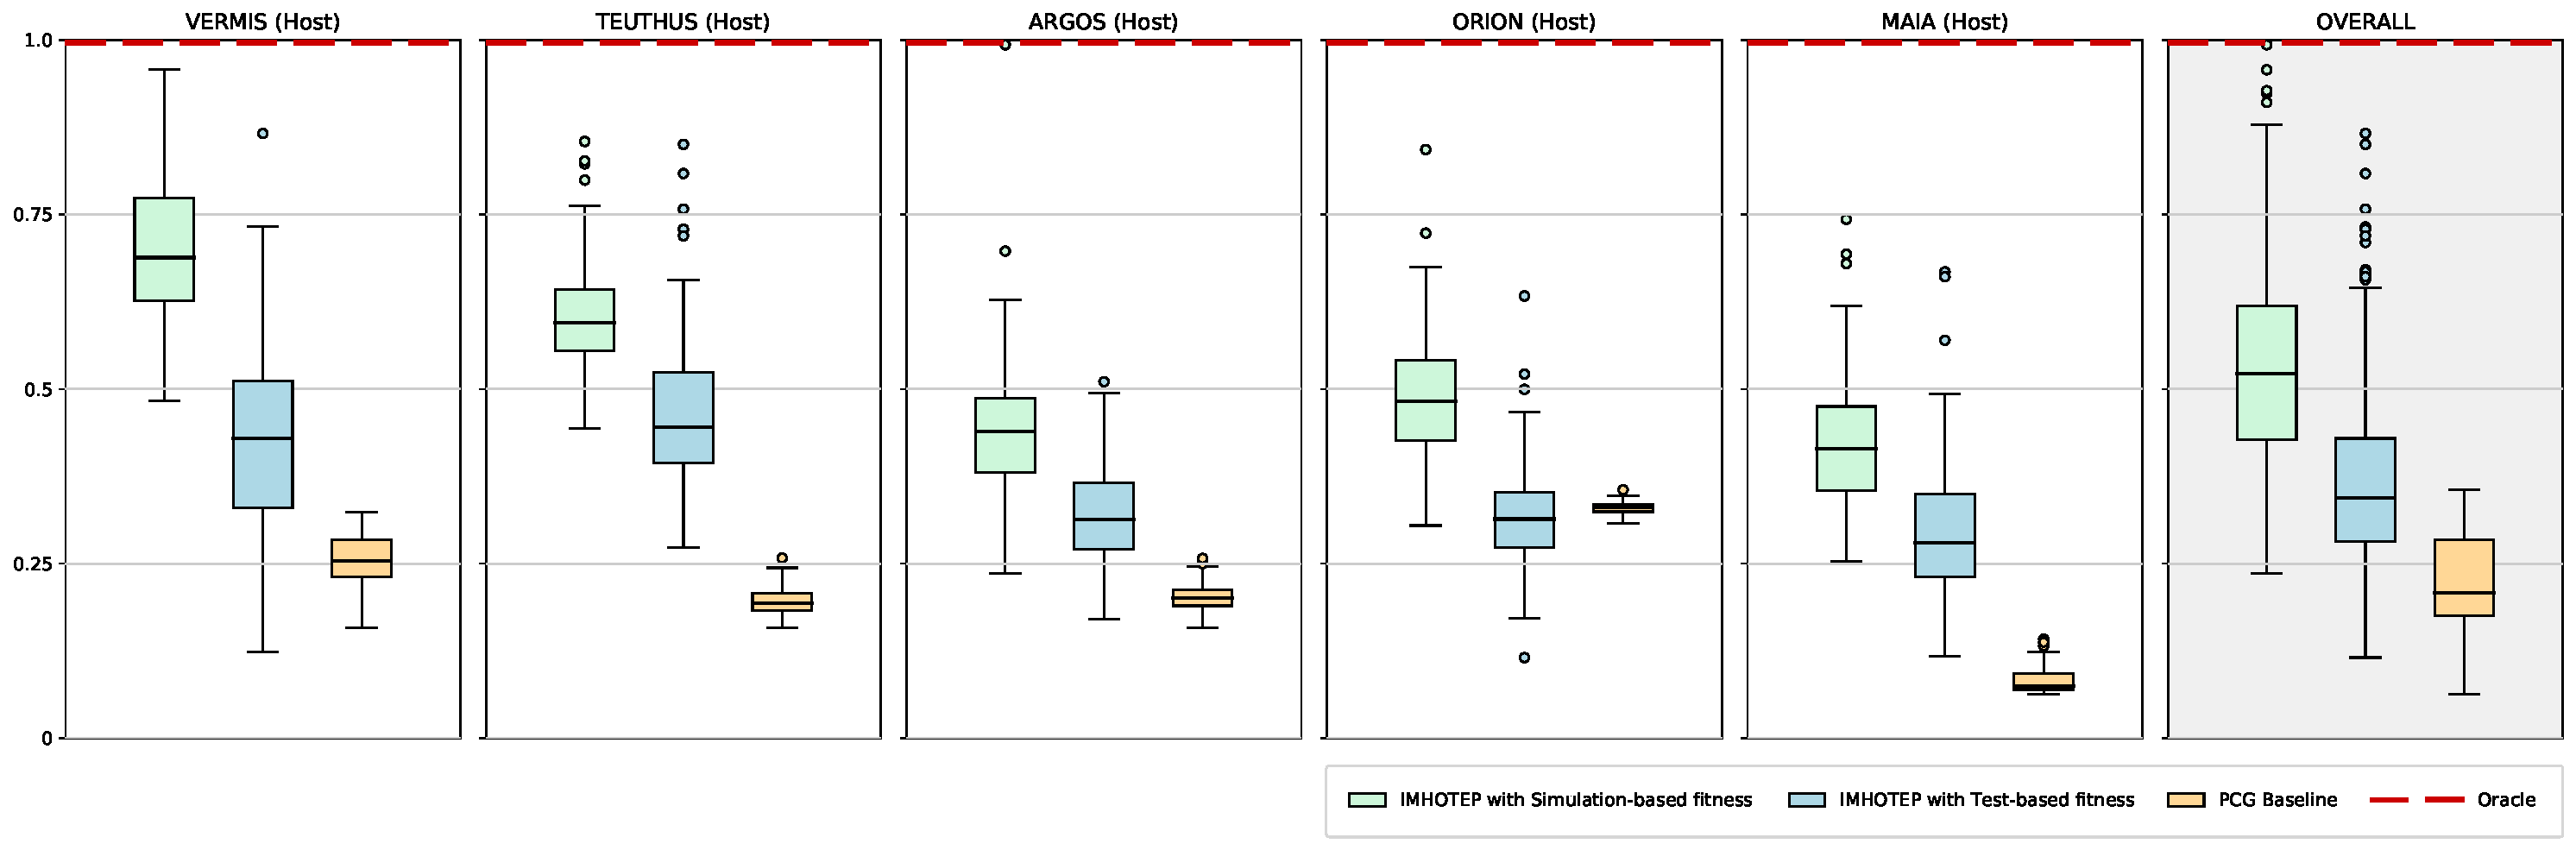
\includegraphics[width=\textwidth]{Figures/Imhotep_with_legend_and_oracle_average-v4.pdf}
    \caption{Results}
    \label{fig:results}
\end{figure*}

% Figure \ref{fig:results} shows the results of the evaluation execution of our approach when using the two objective functions (simulation-Based and test-Based) from \ApproachName{} and the PCG Baseline. The executions are grouped by each host (boss of \CaseStudy{}) that has been used in our experiment (Vermis, Teuthus, Argos, Orion, and Maia). The last column, with shaded background, shows the average of all the hosts for each objective function and the baseline. In addition, the oracle indicates the value obtained by the human-generated final boss models that were obtained from \CaseStudy{}. 

% Each boxplot is generated from the results of each host obtained from the transplantation of each of the 5 hosts with each of the 129 organs. Therefore, each boxplot represents 645 values of a specific host-organ transplantation in a final boss model. Figure \ref{fig:results} shows in each column how the quality values obtained for each of the three strategies studied in our evaluation differ from the values for the models generated by the developers, which are represented by the horizontal red dashed lines that cross each host column. The boxplots that are closer to the horizontal lines are more similar in quality to the models produced by the developers. Additionally, the use of boxplots allows for the representation of the different results for the strategies used.

% To have more detail about the results presented in Figure~\ref{fig:results} we include Table~\ref{tab:mean_sd} and Table~\ref{tab:max_min}. Table~\ref{tab:mean_sd} presents the results of our evaluation in terms of their mean values and their corresponding standard deviation. On other hand, Table~\ref{tab:max_min} shows the maximum and minimum values of the results. On both tables, we have the respective results of each host used in our experiment (Vermis, Teuthus, Argos, Orion, and Maia), and the last column shows the average of all the hosts.

% \textbf{RQ1 answer.} The results in Figure~\ref{fig:results} shows how simulation-based \ApproachName{} variant reaches the closer results to the oracle. Table~\ref{tab:max_min} shows that in two cases (Vermis and Maia) our approach is capable to obtain even better results than the oracle.

% \textbf{RQ2 answer.} Observing Table~\ref{tab:mean_sd} we can notice the difference in quality between our simulation-based and test-based variants. Simulation-based variant obtains 17\% better results than our test-based variant. 

% \textbf{RQ3 answer.} We can draw conclusions about the difference between \ApproachName{} and the baseline from the results of Table~\ref{tab:mean_sd}. The results reveal that simulation-based and test-based variants from our approach compared to the baseline obtain 32\% and 25\% respectively better results than the baseline. Table~\ref{tab:max_min} also reveals how there is a significant difference of 0.93 in the maximum values that simulation-based and the baseline can achieve, and 0.51 comparing test-based and the baseline.

\begin{table*}[t!]
    \caption{Mean Values and Standard Deviations}
    \label{tab:mean_sd}
    \centering
    \resizebox{\textwidth}{!}{%
    \begin{tabular}{llllllll}
    \toprule
    &\multicolumn{1}{c}{Vermis}
    &\multicolumn{1}{c}{Teuthus}
    &\multicolumn{1}{c}{Argos}
    &\multicolumn{1}{c}{Orion}
    &\multicolumn{1}{c}{Maia}
    &\multicolumn{1}{c}{Overall}
    \\ \midrule
    Simulation
    & 0.699 $\pm$ 0.105 & 0.607 $\pm$ 0.074 & 0.439 $\pm$ 0.093 & 0.488 $\pm$ 0.087 & 0.430 $\pm$ 0.121 & 0.533 $\pm$ 0.142       
    \\
    Test
    & 0.424 $\pm$ 0.130 & 0.463 $\pm$ 0.105 & 0.321 $\pm$ 0.069 & 0.314 $\pm$ 0.068 & 0.295 $\pm$ 0.093 & 0.363 $\pm$ 0.117        
    \\
    Baseline
    & 0.254 $\pm$ 0.033 & 0.195 $\pm$ 0.018 & 0.201 $\pm$ 0.018 & 0.329 $\pm$ 0.008 & 0.084 $\pm$ 0.018 & 0.213 $\pm$ 0.083
    \\ \midrule     
\end{tabular}
}
\end{table*}

\begin{table*}[t!]
    \caption{Max and Min values.}
    \label{tab:max_min}
    \centering
    \resizebox{\textwidth}{!}{%
    \begin{tabular}{lllllllllllll}
    \toprule
    & \multicolumn{2}{c}{Vermis}
    & \multicolumn{2}{c}{Teuthus}
    & \multicolumn{2}{c}{Argos}
    & \multicolumn{2}{c}{Orion}
    & \multicolumn{2}{c}{Maia}
    & \multicolumn{2}{c}{Overall}
    \\ \midrule
    \multicolumn{1}{c}{} 
    & \multicolumn{1}{c}{Max} & \multicolumn{1}{c}{Min} 
    & \multicolumn{1}{c}{Max} & \multicolumn{1}{c}{Min} 
    & \multicolumn{1}{c}{Max} & \multicolumn{1}{c}{Min}
    & \multicolumn{1}{c}{Max} & \multicolumn{1}{c}{Min} 
    & \multicolumn{1}{c}{Max} & \multicolumn{1}{c}{Min} 
    & \multicolumn{1}{c}{Max} & \multicolumn{1}{c}{Min} 
    \\
    Simulation & 1.042 & 0.482   & 0.854 & 0.443   & 0.992 & 0.235   & 0.842 & 0.304   & 1.285 & 0.253   & 1.285 & 0.235                          
    \\
    Test & 0.866 & 0.123   & 0.850 & 0.273   & 0.510 & 0.170   & 0.633 & 0.115   & 0.667 & 0.117   & 0.866 & 0.115   
    \\
    Baseline & 0.323 & 0.157   & 0.257 & 0.158   & 0.257 & 0.157   & 0.355 & 0.307   & 0.141 & 0.063    & 0.355 & 0.063
    \\ \midrule                     
\end{tabular}
}
\end{table*}